% RASP final presentation (Beamer, 16:9). Build: latexmk -pdf slides.tex
% Numbers and figures are shared with the report: ../report/generated/*.tex and ../report/figures/
% (scripts/make_report_assets.py). Unmeasured values show as red ??key.
\documentclass[aspectratio=169,11pt]{beamer}
\usetheme{default}
\usecolortheme{dove}
\setbeamertemplate{navigation symbols}{}
\setbeamertemplate{footline}[frame number]
\setbeamerfont{frametitle}{series=\bfseries}
\usepackage[T1]{fontenc}
\usepackage{lmodern}
\usepackage{booktabs}
\usepackage{verbatim}
\usepackage{tikz}
\usetikzlibrary{arrows.meta,positioning}
\definecolor{raspblue}{HTML}{2a78d6}
\definecolor{rasporange}{HTML}{eb6834}
\setbeamercolor{structure}{fg=raspblue}

\graphicspath{{../report/}}
% Report macros. Every result in the report is a \stat{key}: generated/*.tex (scripts/make_report_assets.py) defines
% the values with \setstat{key}{value}. A key without a value prints a red ??key and a LaTeX warning, so a number that
% has not been measured yet (Phases 4-5 before the GPU runs) is impossible to miss.
\makeatletter
\newcommand{\setstat}[2]{\expandafter\def\csname rasp@stat@#1\endcsname{#2}}
\DeclareRobustCommand{\stat}[1]{%
  \ifcsname rasp@stat@#1\endcsname\csname rasp@stat@#1\endcsname
  \else\textcolor{red}{\textbf{??#1}}\PackageWarning{rasp}{No value for `#1' (run scripts/make_report_assets.py)}\fi}
\newcommand{\stattable}[1]{\stat{table:#1}}
% \rfig[width]{name}: figures/name.pdf (or .png), or a visible placeholder until the figure exists.
\newcommand{\rfig}[2][\linewidth]{%
  \IfFileExists{figures/#2.pdf}{\includegraphics[width=#1]{figures/#2.pdf}}{%
    \IfFileExists{figures/#2.png}{\includegraphics[width=#1]{figures/#2.png}}{%
      \fbox{\parbox[c][3.5cm][c]{\dimexpr#1-2\fboxsep-2\fboxrule\relax}{\centering
        \textcolor{red}{\textbf{missing figure: \texttt{\detokenize{#2}}}}\\[2pt]
        \small (produced by \texttt{scripts/make\_report\_assets.py} after the GPU runs)}}}}}
\makeatother
\newcommand{\x}{$\times$}
\newcommand{\G}[1]{\textbf{G#1}}
\newcommand{\todo}[1]{\textcolor{orange}{[TODO: #1]}}

\InputIfFileExists{../report/generated/platform.tex}{}{}
\InputIfFileExists{../report/generated/phase2.tex}{}{}
\InputIfFileExists{../report/generated/phase3.tex}{}{}
\InputIfFileExists{../report/generated/phase4.tex}{}{}
\InputIfFileExists{../report/generated/phase5.tex}{}{}
% \rfig looks in figures/ relative to the report; point it there from here.
\renewcommand{\rfig}[2][\linewidth]{%
  \IfFileExists{../report/figures/#2.pdf}{\includegraphics[width=#1]{../report/figures/#2.pdf}}{%
    \IfFileExists{../report/figures/#2.png}{\includegraphics[width=#1]{../report/figures/#2.png}}{%
      \fbox{\parbox[c][3cm][c]{\dimexpr#1-2\fboxsep-2\fboxrule\relax}{\centering
        \textcolor{red}{\textbf{figure \texttt{\detokenize{#2}}}}\\ \small (after the GPU runs)}}}}}

\title{RASP: Runtime-Adaptive Sparse Matrix Kernels on a PCIe GPU}
\subtitle{Choosing SpMV formats and out-of-core SpGEMM schedules per matrix, at run time}
\author{Harsh Raj \and Karmanya \and \todo{third member}}
\date{\todo{course} \quad December 2026}

\begin{document}

\begin{frame}
\titlepage
\end{frame}

\begin{frame}{The problem: sparse kernels have no single best implementation}
\begin{itemize}
\item SpMV and SpGEMM are memory-bound and irregular: row-length spread, the longest row and the operand sizes
  relative to GPU memory decide what is fastest.
\item Both papers we build on \textbf{measure} this, then ship a \textbf{static} choice:
  \begin{itemize}
  \item Heller \& Oberhuber 2012 (ArgCSR): one global \texttt{desiredChunkSize} for every matrix.
  \item Deveci et al.\ 2018 (out-of-core SpGEMM): a fixed 75/25 split of fast memory, chosen by copy volume,
    no copy/compute overlap.
  \end{itemize}
\item \textbf{RASP decides at run time, per matrix, from cheap measurements}:
  \begin{enumerate}
  \item SpMV: GPU features $\to$ decision tree $\to$ conversion break-even.
  \item SpGEMM: measured PCIe and kernel rates $\to$ simulated pipeline plan $\to$ re-plan while running.
  \end{enumerate}
\item Platform: RTX 4050 Laptop (Ada, 6\,GB) over PCIe 4.0 x8, WSL2.
\end{itemize}
\end{frame}

\begin{frame}{Paper 2 on 2026 hardware: the sensitivity reproduces, the headline does not}
\begin{columns}[T]
\column{0.5\textwidth}
\rfig{p2_argcsr_chunk}
\column{0.48\textwidth}
\begin{itemize}
\item \texttt{rajat23}: chunk size 1 gives \stat{p2-rajat23-d1} GFLOP/s, 32 gives \stat{p2-rajat23-d32} (paper: 5.1 vs 0.81):
  padding grows \stat{p2-rajat23-stored-d1}\x$\to$\stat{p2-rajat23-stored-d32}\x.
\item A global chunk size 1 is best on \stat{p2-d1-best-count-fp64} of \stat{p2-matrices} matrices and costs
  \stat{p2-d1-slowdown}\x{} on average (worst \stat{p2-d1-worst}\x).
\item ArgCSR vs cuSPARSE \texttt{ALG1}: \stat{p2-argcsr-default-fp64}\x{} at default, \stat{p2-argcsr-tuned-fp64}\x{}
  tuned (fp64). Not ``10\x{} faster'' anymore.
\end{itemize}
\end{columns}
\end{frame}

\begin{frame}{No format wins everywhere, but the margin over cuSPARSE is thin}
\begin{columns}[T]
\column{0.62\textwidth}
\rfig{p2_perf_profile}
\column{0.36\textwidth}
\begin{itemize}
\item Oracle over \stat{p2-configs} configs: \stat{p2-oracle-fp32}\x{} (fp32), \stat{p2-oracle-fp64}\x{} (fp64)
  vs cuSPARSE.
\item Headroom lives in small matrices: \stat{p2-oracle-size-lt100k}\x{} below $10^5$ nnz,
  \stat{p2-oracle-size-gt1M}\x{} above $10^6$.
\item Our ArgCSR-local (chunk size per row region): \stat{p2-local-vs-default}\x{} over paper 2's default, untuned.
\end{itemize}
\end{columns}
\end{frame}

\begin{frame}{RASP for SpMV: \texttt{SpmvPlan(A, x, y, \{expected\_calls = N\})}}
\centering
\resizebox{\textwidth}{!}{%
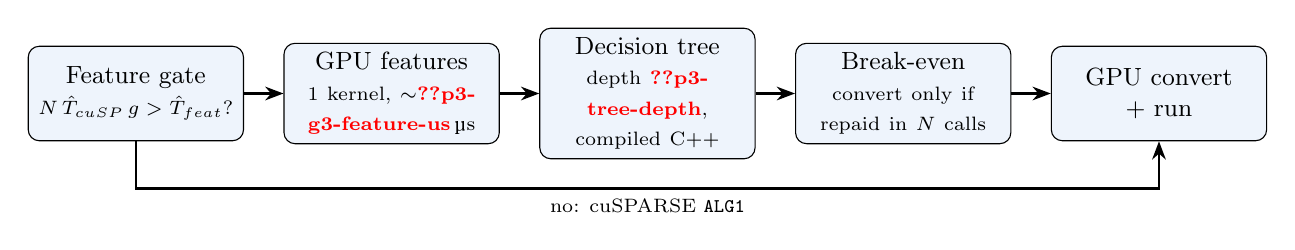
\begin{tikzpicture}[node distance=7mm and 5mm, box/.style={draw, rounded corners, fill=raspblue!8, align=center,
  minimum height=12mm, text width=25mm, font=\small}, arr/.style={-{Stealth}, thick}]
\node[box] (gate) {Feature gate\\{\scriptsize $N\,\hat T_\text{cuSP}\,g > \hat T_\text{feat}$?}};
\node[box, right=of gate] (feat) {GPU features\\{\scriptsize 1 kernel, $\sim$\stat{p3-g3-feature-us}\,\textmu s}};
\node[box, right=of feat] (tree) {Decision tree\\{\scriptsize depth \stat{p3-tree-depth}, compiled C++}};
\node[box, right=of tree] (be) {Break-even\\{\scriptsize convert only if repaid in $N$ calls}};
\node[box, right=of be] (build) {GPU convert\\+ run};
\draw[arr] (gate) -- (feat); \draw[arr] (feat) -- (tree); \draw[arr] (tree) -- (be); \draw[arr] (be) -- (build);
\draw[arr] (gate.south) -- ++(0,-6mm) -| node[pos=0.25, below, font=\scriptsize]{no: cuSPARSE \texttt{ALG1}} (build.south);
\end{tikzpicture}}
\vspace{4mm}
\begin{itemize}
\item Trained on \stat{p3-train-matrices} matrices; 5-fold CV \emph{grouped by SuiteSparse group}; portfolio of 5
  configs within \stat{p3-cv-portfolio}\x{} of the full oracle; large-matrix gate chosen by CV.
\item GPU converters (bit-identical to host): ArgCSR \stat{p3-gpu-convert-calls-argcsr}, SELL
  \stat{p3-gpu-convert-calls-sell}, CSR-binned \stat{p3-gpu-convert-calls-csr-binned} SpMVs.
\end{itemize}
\end{frame}

\begin{frame}{G2--G4 on \stat{p3-heldout-matrices} unseen matrices}
\begin{columns}[T]
\column{0.5\textwidth}
\rfig{p3_oracle_gap}
\column{0.48\textwidth}
\begin{itemize}
\item \textbf{G2 met:} tree at \stat{p3-g2-tree}\x{} of the oracle (target $\le$1.10), \stat{p3-g2-tree-vs-cusparse}\x{}
  vs cuSPARSE, \stat{p3-g2-tree-slower-large} losses on large matrices.
\item Hand-written rules: \stat{p3-g2-rules}\x{} -- no better than cuSPARSE (\stat{p3-g2-cusparse}\x).
\item \textbf{G3 borderline:} features cost \stat{p3-g3-median} SpMVs (median), \stat{p3-g3-size-gt1M} for large
  matrices.
\item \textbf{G4 met:} at $N=1$ \stat{p3-g4-tree-1}\x{} of cuSPARSE (without break-even:
  \stat{p3-g4-tree-nobe-1}\x); at $N=1000$ \stat{p3-g4-tree-1000}\x.
\end{itemize}
\end{columns}
\end{frame}

\begin{frame}{Out-of-core SpGEMM on PCIe: what changes vs paper 1}
\begin{itemize}
\item Paper 1: \textbf{chunk1} keeps $A$/$C$ rows resident and streams $B$; \textbf{chunk2} keeps $B$ rows resident and
  streams $A$/$C$. Alg.~4: 75\% / 25\% of fast memory, variant by copy volume, \textbf{no overlap}.
\item Our link: \stat{pf-h2d} GB/s PCIe vs \stat{pf-device-read} GB/s device (1:\stat{pf-stream-penalty}),
  \textbf{one copy engine} (H2D + D2H together: \stat{pf-bidir} GB/s).
\item WSL2: managed memory never migrates: UVM $\equiv$ zero-copy (\stat{pf-uvm-read} vs \stat{pf-zc-read} GB/s).
\end{itemize}
\vspace{2mm}
\begin{block}{G5: each operand in pinned memory (slowdown vs all-device)}
\centering\small\stattable{p4-placement}
\end{block}
\end{frame}

\begin{frame}{RASP for SpGEMM: \texttt{SpgemmContext(budget).multiply(A, B, C)}}
\begin{itemize}
\item \textbf{Measure:} PCIe bandwidth at start-up; flop count and $\mathrm{nnz}(C)$ bound per row (one host pass).
\item \textbf{Plan by simulation:} every mode (in-core, zero-copy, chunk$B$ 1-D / multi-block, chunk$AC$) $\times$
  block sizes $\times$ depth 2--3, scored by simulating the issue order on one copy engine; the streamed operand
  gets \emph{all} memory the resident one leaves (not 25\%).
\item \textbf{Calibrate:} a small probe block measures kernel rate, compression $\gamma$ and cuSPARSE workspace;
  re-partition the rows not yet uploaded when any drifts $>$20\%.
\item \textbf{Execute:} copy stream + compute stream, uploads $d-1$ tiles ahead; every buffer from one budget arena
  (peak $\le$ budget, always); tiles that do not fit are split and redone.
\end{itemize}
\end{frame}

\begin{frame}{G6: RASP vs paper 1's Algorithm 4}
\begin{columns}[T]
\column{0.6\textwidth}
\rfig{p4_scaling}
\column{0.38\textwidth}
\begin{itemize}
\item Problem $>$ budget: \stat{p4-g6-AxP}\x{} ($A\cdot P$), \stat{p4-g6-RxA}\x{} ($R\cdot A$) over Alg.~4
  (target 1.3).
\item Cost model: predicted / measured \stat{p4-model-accuracy}; estimate + plan \stat{p4-overhead-pct}\% of the time.
\end{itemize}
\vspace{2mm}
{\small\stattable{p4-ablation}}
\end{columns}
\end{frame}

\begin{frame}{Where the time goes: copy engine vs compute}
\centering\rfig[0.9\textwidth]{p4_timeline}
\end{frame}

\begin{frame}{G7: end-to-end applications}
\begin{columns}[T]
\column{0.5\textwidth}
\textbf{CG} (Jacobi-preconditioned, \stat{p5-cg-matrices} SPD matrices; hint = iteration cap)
\begin{itemize}
\item Time-to-solution vs cuSPARSE: \stat{p5-cg-tree-geomean}\x{} (worst \stat{p5-cg-tree-worst}\x)
\item With the exact iteration count: \stat{p5-cg-tree-exact-geomean}\x
\item SpMV is \stat{p5-cg-spmv-share}\% of a solve
\end{itemize}
\column{0.48\textwidth}
\textbf{AMG set-up} $A_{l+1} = R_l(A_lP_l)$, Laplace3D $n=192$, 256\,MiB budget
\vspace{1mm}

{\small\stattable{p5-amg-192}}
\end{columns}
\end{frame}

\begin{frame}[fragile]{Live demo: \texttt{./build/rasp\_demo}}
\IfFileExists{../../results/phase5/demo.txt}{%
  {\tiny\verbatiminput{../../results/phase5/demo.txt}}}{%
  \begin{itemize}
  \item \texttt{rajat23} (circuit) vs \texttt{af\_shell1} (FEM): features, the plan at $N = 1, 100, 10\,000$ and why,
    plan + $N$ calls vs cuSPARSE.
  \item Laplace $A\cdot P$ under a budget: Alg.~4 vs RASP plans, times, measured model, first pipeline tiles.
  \item \textcolor{red}{transcript appears here after \texttt{scripts/run\_phase5.sh}}
  \end{itemize}}
\end{frame}

\begin{frame}{Conclusions}
\begin{itemize}
\item Both papers measured the right thing and then fixed a choice; RASP makes it at run time.
\item SpMV: \stat{p3-g2-tree}\x{} of the oracle on unseen matrices, never costlier than cuSPARSE for one call --
  break-even is what makes a selector safe.
\item SpGEMM: measured, simulated and re-planned schedules with overlap: \stat{p4-g6-AxP}\x{} / \stat{p4-g6-RxA}\x{}
  over Alg.~4 out of core.
\item Re-evaluation: ArgCSR's chunk-size sensitivity holds; its lead over the vendor library does not.
\item Limits: one laptop GPU under WSL2 (no real UVM), \stat{p3-heldout-large} large held-out matrices, G3 borderline,
  cuSPARSE as SpGEMM engine.
\end{itemize}
\end{frame}

\end{document}
